\subsubsection{\stid{2.02} LANL ATDM Tools}

\paragraph{Overview}
The Los Alamos National Laboratory ATDM Tools project provides tools
and software infrastructure for improving various aspects of the
Exascale programming environment.  At present our efforts are
primarily focused on an advanced LLVM~\cite{LLVM:2018} compiler and
tool infrastructure supporting a new explicit parallel intermediate
representation for the C/C++ and Fortran programming languages.  These
efforts also include interactions with the broader LLVM community and
several platform vendors (e.g. NVIDIA and ARM).  This work also covers
a set of interactions and engagements focused on collaboration with the
Flang project (ST 2.3.5.06) with a goal of providing a long-term Fortran
language capability within the LLVM infrastructure. 

\paragraph{Key Challenges}
One fundamental challenge for our efforts is planning for and
providing system architectures that yet to be completed defined in a
manner that makes them a well-defined target for compilation.  This
risk is likely significantly mitigated given the wide use and adoption
of LLVM across the many key system and processor vendors.  Additional
challenges stem from the adoption of our designs and implementations
into the overall LLVM community -- given their broader and more
general focus.  

\paragraph{Solution Strategy}
Given the project challenges, our approach considers aspects of
today's node-level programming systems (e.g. OpenMP and Kokkos) and
popular programming languages (e.g. C++ and Fortran) into
consideration and aims to improve and expand upon their capabilities
to address the needs of ECP.  This allows us to attempt to strike a
balance between incremental improvements to existing infrastructure
along with more aggressive techniques that seeks to provide innovative
solutions to help both manage risk and the ability to introduce new
breakthrough technologies.

To mitigate some aspects of risk, we are working to form close working
relationships with the LLVM community to help provide an impact and
longer term set of technologies to the broader computing community.
These activities span both academic and industry collaborations.

\paragraph{Recent Progress}
Our most recent efforts have focused on supporting an infrastructure
that maps multiple language constructs from Kokkos, FleCSI and OpenMP
into an common intermediate representation that explicitly captures
the parallel operations for analysis and optimization (this is a
capability that does not exist in the mainline LLVM infrastructure).
This parallel representation may then also be targeted to different
runtime systems (not necessarily those of use by the programming
system used in the original source programs).  See our most recent
paper for a discussion of our overall approach~\cite{Stelle:2017}.  In
addition, this work will be presented at the upcoming EuroLLVM
workshop~\cite{EuroLLVM:2018}.  We will continue to reach out to the
broader LLVM community via such events to provide updates and share the
lessons learned and example use cases of this technology.  Most recently,
at the US LLVM Developer's Meeting, an RFC for was released for
adding parallel intrinsics to LLVM as a collaboration between LANL,
MIT, ANL, Intel, and UIUC~\cite{LLVMPAR:rfc}.

In addition to runtime improvements, we've shown that by compiling
directly to parallel IR instead of the codepath based on C++
template explansion for Kokkos we can gain significant improvements in
overall application compile time and a significant reduction in binary
size. See Figure~\ref{fig:2.3.2.02:time_size} for quantification of the compile
time speedup and binary size reduction.

\begin{figure}
  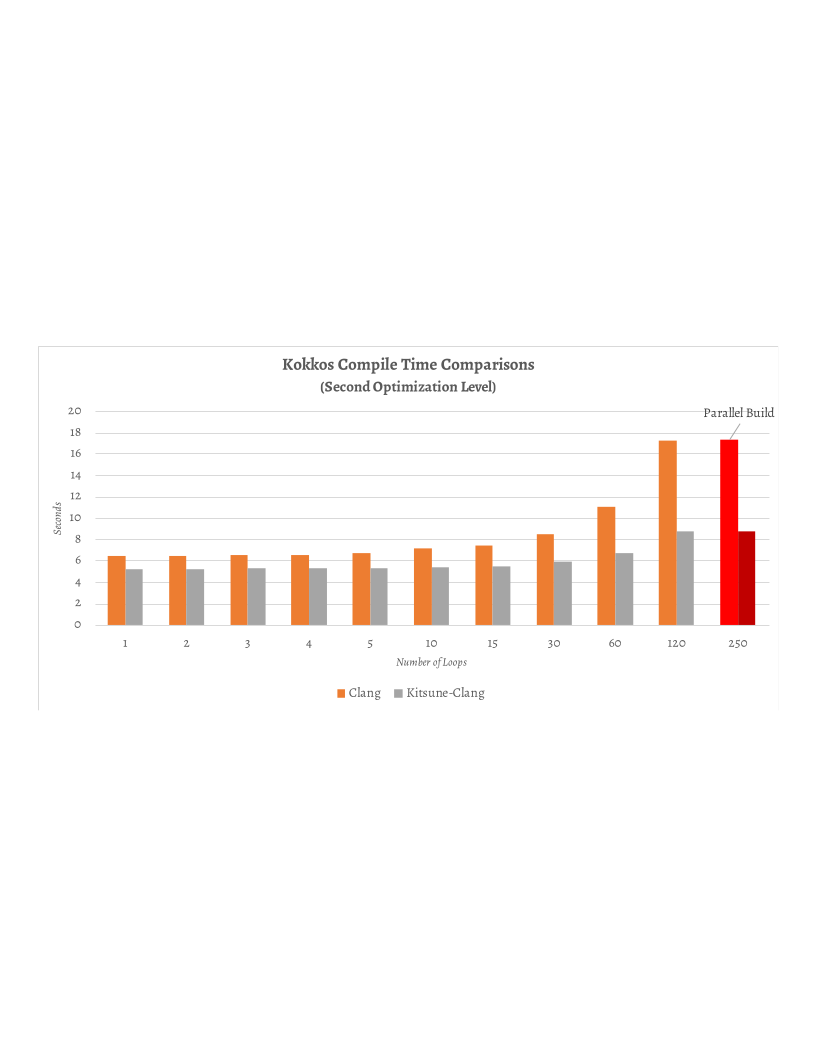
\includegraphics[width=0.8\textwidth]{projects/2.3.2-Tools/2.3.2.02-LANL-ATDM-Tools/kokkos-compile-times.png}
  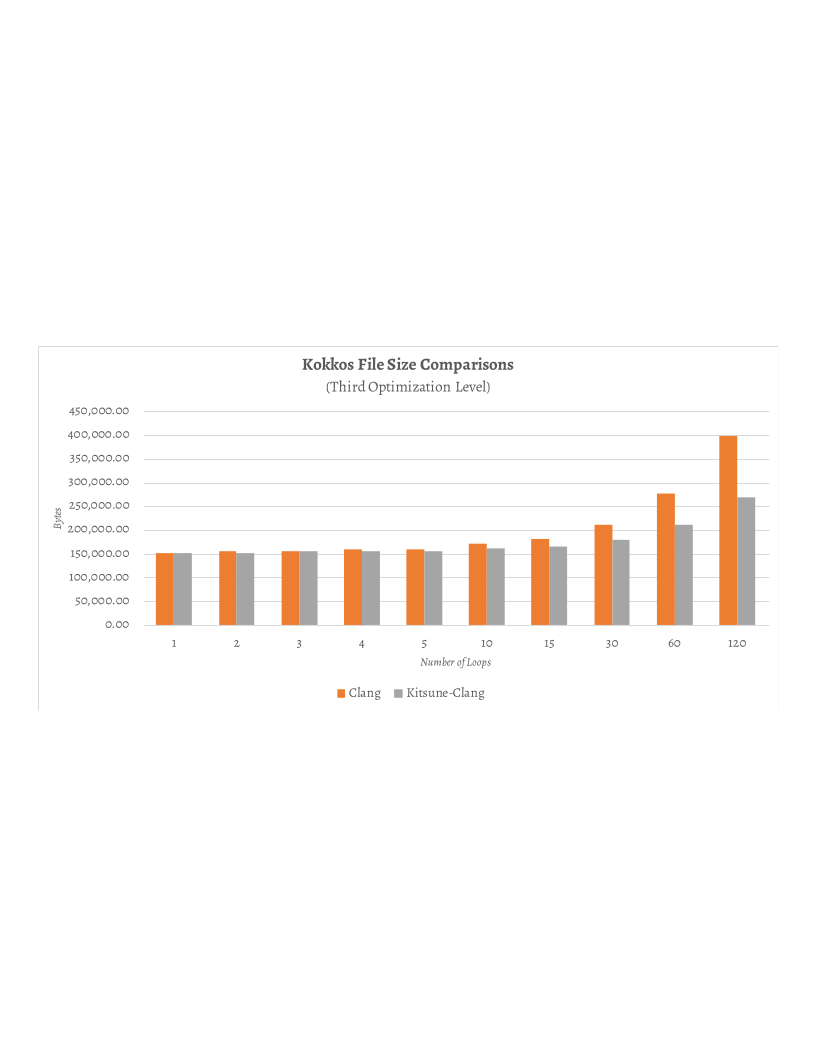
\includegraphics[width=0.8\textwidth]{projects/2.3.2-Tools/2.3.2.02-LANL-ATDM-Tools/kokkos-file-size.png}
  \caption{Compile time improvements and object file size reductions for
           Kokkos applications with an increasing number of parallel-for
           looping constructs.}
  \label{fig:2.3.2.02:time_size}                      
\end{figure}


\paragraph{Next Steps}
The Kitsune efforts are highlighed by a series of quarterly milestones
and associated software releases throughout the coming year.  The
Kitsune compiler is still very much an active \emph{proof-of-concept}
compiler toolchain focused on C and C++ with plans to soon add support
for Fortran via the Flang project~\cite{Flang:2018}.  Even though it
is not yet production ready we are actively releasing source code and
the supporting infrastructure for deployment as an exploratory and
early evaluation candidate.  These efforts will all continue to
include significant interactions and collaborations with the other ECP
efforts surrounding LLVM and also engage with the broader LLVM and
vendor communities on our assocaited technology.
